% Compile with pdfLaTeX. All content, tables and the workflow are editable here.
% Source: Phase2_Report10/Phase2_Report10 (1).tex, unchanged.
\documentclass[aspectratio=169,11pt]{beamer}
\usepackage[utf8]{inputenc}
\usepackage[T1]{fontenc}
\usepackage{lmodern}
\usepackage{amsmath,amssymb,booktabs,array,graphicx,tikz}
\usetikzlibrary{arrows.meta}
\definecolor{ink}{HTML}{14314A}
\definecolor{accent}{HTML}{007F89}
\definecolor{muted}{HTML}{506371}
\setbeamercolor{normal text}{fg=ink,bg=white}
\setbeamercolor{frametitle}{fg=ink,bg=white}
\setbeamercolor{title}{fg=ink}
\setbeamercolor{structure}{fg=accent}
\setbeamercolor{alerted text}{fg=accent}
\setbeamerfont{frametitle}{size=\Large,series=\bfseries}
\setbeamerfont{title}{size=\LARGE,series=\bfseries}
\setbeamersize{text margin left=9mm,text margin right=9mm}
\setbeamertemplate{navigation symbols}{}
\setbeamertemplate{headline}{}
\setbeamertemplate{footline}{\hfill\usebeamercolor[fg]{structure}\scriptsize
  \insertframenumber\hspace{9mm}\vspace{3mm}}
\setbeamertemplate{itemize item}{\small\textbullet}
\setlength{\parskip}{6pt}
\newcolumntype{L}[1]{>{\raggedright\arraybackslash}p{#1}}
\newcommand{\smallnote}[1]{\par{\footnotesize\color{muted}#1\par}}
\title{Course Registration Helper\\for Balanced Workloads}
\subtitle{Phase 2: AI Project Presentation}
\author{}
\date{}
\hypersetup{pdftitle={Course Registration Helper for Balanced Workloads},pdfauthor={}}

\begin{document}

% 01 -- Cover
\begin{frame}[plain]
\vspace{10mm}
{\color{accent}\large Phase 2: AI Project Presentation\par}
\vspace{5mm}
{\usebeamerfont{title}Course Registration Helper\\for Balanced Workloads\par}
\vspace{7mm}
{\large Personalised course rewards and external path optimisation\par}
\end{frame}

% 02 -- Introduction
% 02 -- Introduction
\begin{frame}{Introduction}
Study-path planning is an important process in university life, yet it is often rushed due to:
\begin{itemize}\setlength{\itemsep}{4pt}
\item Unfamiliarity with GE and elective-course backgrounds or workloads
\item Limited seats and short add/drop periods
\end{itemize}
There is a common example that:
\vspace{1mm}
\begin{center}
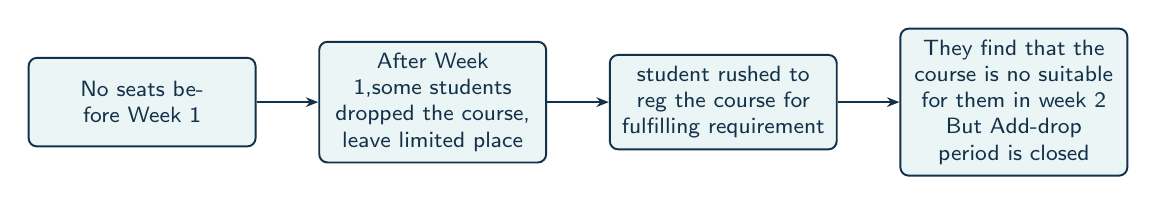
\begin{tikzpicture}[
    x=1pt, y=1pt,
    box/.style={
        rectangle,
        draw=ink,
        line width=0.7pt,
        rounded corners=3pt,
        fill=accent!8,
        text=ink,
        text width=74pt,
        minimum height=32pt,
        inner sep=4pt,
        align=center,
        font=\sffamily\footnotesize
    },
    arrow/.style={
        -{Stealth[length=4.5pt, width=3.5pt]},
        line width=0.7pt,
        draw=ink
    }
]
    % Nodes positioned explicitly
    \node[box] (n1) at (0,0)   {No seats before Week 1};
    \node[box] (n2) at (105,0) {After Week 1,some students dropped the course,\\leave limited place };
    \node[box] (n3) at (210,0) {student rushed to reg the course for fulfilling requirement};
    \node[box] (n4) at (315,0) {They find that the course is no suitable for them in week 2\\ But Add-drop period is closed};

    % Direct Arrows
    \draw[arrow] (n1.east) -- (n2.west);
    \draw[arrow] (n2.east) -- (n3.west);
    \draw[arrow] (n3.east) -- (n4.west);
\end{tikzpicture}
\end{center}
\vspace{1mm}
Our helper aims to suggest the suitable workload-aware schedule,by using students' interests, profile,by a fine-tuned LLM and mathematical optimisation problem

\end{frame}


% 03 -- Data
\begin{frame}{Method:data for fine-tunning}
We fine-tune a LLM with:\\
Handbook, CM path/course list, CS major and suggested path way in website, GE's information, saved Semester A/B timetables, course's information
\vspace{2mm}
\begin{tabular}{L{9.4cm}r}
\toprule
Timetable PDFs collected & 93\\
Successfully parsed / excluded & 86 / 7\\
Timetable PDFs represented in programme training & 82\\
Programme PDFs represented in programme training & 3\\\midrule
\textbf{PDF sources represented in the 485-example split} & \textbf{85}\\
\bottomrule
\end{tabular}\par
\vspace{2mm}
We train on extracted text and facts as JSON: course identities, credits, prerequisites, exclusions, restrictions and meetings.

\end{frame}

% 04 -- Fine tuning and prompts
\begin{frame}{Qwen learns a structured reward policy}
Qwen3-8B uses rank-8 QLoRA, a frozen four-bit base and BF16 computation.
\vspace{1mm}
\begin{tabular}{L{7.5cm}L{4.8cm}}
\toprule
Training stage & Examples\\\midrule
Programme data & 485 train / 24 validation / 30 test\\
CM background update & 244 / 32, plus 20 held-out checks\\
Relation distillation & 149 / 20\\
Maximum-versus-sum correction & 82 corrective examples\\
\bottomrule
\end{tabular}\par
\vspace{2mm}
Prompts combine system instructions with student facts/states. Assistant JSON targets use assistant-only cross-entropy loss.
\smallnote{The current prompt allows only \texttt{reward\_parameters} and \texttt{course\_relations}. One local inference exported all eight settings and 26 links without fallback. This tests policy export, not independent reward quality.}
\end{frame}

% 05 -- Workflow, retaining the report's human feedback loop
\begin{frame}{Full workflow: GPT as teacher in begin stages with human feedback}
\centering
\resizebox{\linewidth}{!}{%
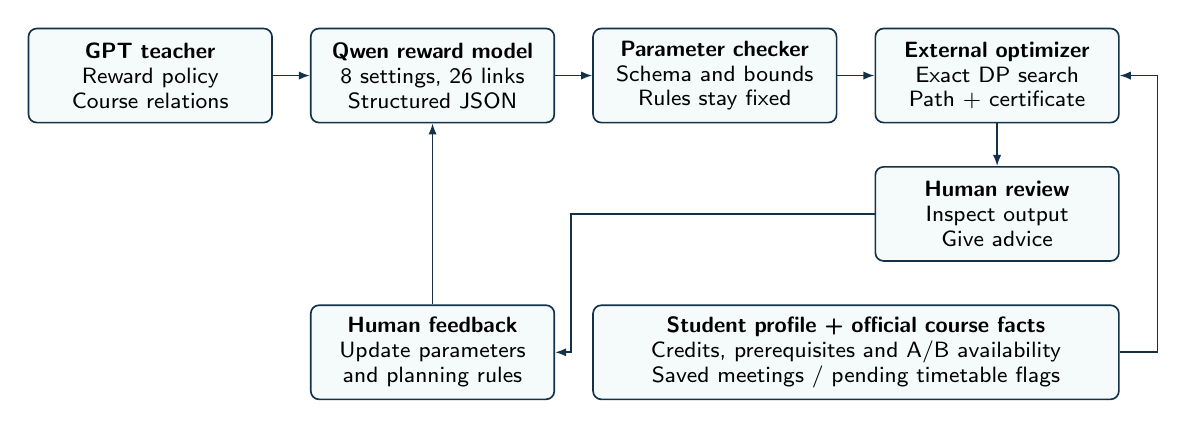
\begin{tikzpicture}[
 x=1pt,y=1pt,
 flowbox/.style={draw=ink,fill=accent!4,rounded corners=3pt,
 line width=.6pt,align=center,text width=82pt,minimum height=34pt,
 inner sep=3pt,font=\sffamily\fontsize{8}{9}\selectfont},
 flowarrow/.style={-{Latex[length=4pt,width=3pt]},draw=ink,line width=.6pt}]
\node[flowbox] (teacher) at (47,117)
 {\textbf{GPT teacher}\\Reward policy\\Course relations};
\node[flowbox] (qwen) at (149,117)
 {\textbf{Qwen reward model}\\8 settings, 26 links\\Structured JSON};
\node[flowbox] (checker) at (251,117)
 {\textbf{Parameter checker}\\Schema and bounds\\Rules stay fixed};
\node[flowbox] (optimizer) at (353,117)
 {\textbf{External optimizer}\\Exact DP search\\Path + certificate};
\draw[flowarrow] (teacher.east)--(qwen.west);
\draw[flowarrow] (qwen.east)--(checker.west);
\draw[flowarrow] (checker.east)--(optimizer.west);
\node[flowbox] (human) at (353,67)
 {\textbf{Human review}\\Inspect output\\Give advice};
\node[flowbox] (feedback) at (149,17)
 {\textbf{Human feedback}\\Update parameters\\and planning rules};
\node[flowbox,text width=184pt] (facts) at (302,17)
 {\textbf{Student profile + official course facts}\\
 Credits, prerequisites and A/B availability\\Saved meetings / pending timetable flags};
\draw[flowarrow] (feedback.north)--(qwen.south);
\draw[flowarrow] (optimizer.south)--(human.north);
\draw[flowarrow] (human.west)--(199,67)--(199,17)--(feedback.east);
\draw[flowarrow] (facts.east)--(411,17)--(411,117)--(optimizer.east);
\end{tikzpicture}}
\vspace{3mm}
\raggedright
GPT teaches course relations and rewards. Fictional examples and human advice guide retraining or planning-rule updates after output review.
\end{frame}
% why LLM
\begin{frame}{Why LLM teacher and why Qwen as input ?}
\textbf{Why we use GPT as teacher in the beginning?}\\
Mainly to save the labor time for primary relation between courses 
\\e.g: the relation between "GE2340 AI:Past,Present,and Future" and "CS4487 Machine Learning"\\
\textbf{Why use qwen LLM as based}\\
We want the iinput becomes more user-friendly and is not limited (by the auto-encoder)\\
However, we will discuss whether the LLM part can be reduced by some other method
\end{frame}
% 06 -- Hardware
\begin{frame}{Hardware details on training}
Here is some information about hardware during training
\textbf{NVIDIA GeForce RTX 5090: 31.82 GiB total CUDA device memory.}
\vspace{1mm}
\begin{tabular}{L{9cm}r}
\toprule
Separate training run & Peak allocated GiB\\\midrule
Programme training & 8.27\\
Finance-background update & 7.37\\
Relation correction & 8.35\\
Longer-context degree-policy update & 15.84\\\midrule
Representative inference & 5.99\\
\bottomrule
\end{tabular}\par
\smallnote{Training: one example per microbatch, accumulation over four examples, 4,096-token contexts (6,144 for degree policy). Inference: batch 1, 598-token prompt, 33-token response; loaded allocation 5.74 GiB and peak reserved 6.10 GiB. Measurements cover this process's PyTorch memory, excluding other apps and driver memory. Context and batch size affect consumption. Python path search runs on CPU.}
\end{frame}
%% Details part
% 07 -- Hard constraints
\begin{frame}{Basic rules forced the output}
\begin{itemize}\setlength{\itemsep}{5pt}
\item At least \textbf{122 unique credits}
\item Four distributional GEs covering Areas 1--3, with at most one per semester. Compulsory language/development GE is separate.
\item fulfilling minimum requirement of elective that required 
\item Mandatory/core courses, project, free electives and chosen stream complete.
\item Each term has zero to six positive-credit courses and at most 18 credits.
\end{itemize}
\smallnote{Courses must appear in the student's designated programme document or the verified GE collection. High reward cannot compensate for missing required credits.}
\end{frame}

% 08 -- Penalty becomes reward
\begin{frame}{Penalty and reward function}
Original weighted penalty for binary course choices $x_i$:
\[
\min_{\mathbf x\in\mathcal X}P(\mathbf x),\qquad
P(\mathbf x)=\sum_i x_i(\lambda_b b_i+\lambda_d d_i+\lambda_w w_i).
\]
Adding course value $R_i$ gives the net-reward objective:
\[
\max_{\mathbf x\in\mathcal X}\left[\sum_i x_iR_i-P(\mathbf x)\right].
\]
\vspace{1mm}
Students adjust non-negative weights for background mismatch ($\lambda_b$), difficulty ($\lambda_d$) and workload ($\lambda_w$).
However,it can be idenify as a markov reward process in the following
\end{frame}

% 09 -- State dependent reward
\begin{frame}{(Final) State-dependent reward function. }
The helper try find a policy path,to maximize
\begin{align*}
U(X,s)={}&\sum_{c\in X}\bigl[g_c(s)+p_c(s)+h_c(s)+q_c(s)+z_c(s)\\
 &-\lambda_b(b_c(s)+e_c(s))-\lambda_d d_c(s)-\lambda_w w_c(s)\bigr]\\
 &+R_{\mathrm{stream}}(X,s)-O(X,s).
\end{align*}
\begin{tabular}{L{6.2cm}L{6cm}}
$g$: base course value & $p$: preparation from earlier study\\
$h$: core priorities & $q$: prerequisite bridges\\
$z$: quota/timing bonuses & $R_{\mathrm{stream}}$: stream progress\\
\\$O(X,s)$:over workload penalty function
\end{tabular}\par
\vspace{2mm}
Claiming one selected stream earns 6 once, multiplied by the student's stream weight.
\smallnote{These scores are configured estimates, not measured study hours.}
\end{frame}

% 10 -- Overload
\begin{frame}{Overload penalty $O(X,s)$}
we don't want the model to advice toomany course in same semster,so we introduce  over workload penalty function $O(X,s)$ 
\[
O(X,s)=\begin{cases}
0.25[\max(0,C(X)-15)]^2,&\text{Years 1--3},\\[6pt]
0.25[\max(0,C(X)-12)]^2,&\text{Year 4}.
\end{cases}
\]
\vspace{3mm}
The 18-credit maximum remains a separate hard constraint.

Term loads stay flexible. A 12- or 13-credit term is valid when the full path reaches 122 credits and satisfies the degree audit.
\smallnote{There is no five-course minimum in every term.}
\end{frame}

% 11 -- Optimisation program
\begin{frame}{Python dynamic programming finds the largest reward}
\begin{enumerate}\setlength{\itemsep}{7pt}
\item Start with completed courses and fixed allocations.
\item Explore permitted semester placements of remaining courses.
\item Update student state in semester order and calculate total discounted reward.
\item Merge identical partial allocations to avoid repeated calculations.
\item Compare feasible completions and return the largest objective value.
\end{enumerate}
\smallnote{The maximum applies to the supplied choices. Qwen provides validated parameters and relations; the external program performs path selection. The latest optimiser revision did not retrain neural weights.}
\end{frame}

\begin{frame}{comparing:GPT test without optimisation tools}
We wish to compare other method to GPT 's direct generating result,where in the following
\begin{itemize}\setlength{\itemsep}{7pt}
\item Direct GPT receives the same parameter packet and course facts.
\item GPT uses no solver, code or browsing, and sees no optimiser answers or scores.
\item A common critic checks the final outputs, with no repair or fallback for GPT.
\end{itemize}

\end{frame}
% 12 -- Blind test profiles
\begin{frame}{Result:Three fictional profiles form the blind comparison}
Each student passes exactly 15 credits in Year 1A and 15 in Year 1B.
\vspace{1mm}
\begin{tabular}{lL{3cm}L{3cm}L{4cm}}
\toprule
Profile & Year 1A GE & Year 1B GE & Desired stream\\\midrule
F & GE2260, Area 2 & GE1105, Area 1 & Financial Mathematics\\[4pt]
N & GE1305, Area 3 & GE1113, Area 1 & Financial Mathematics\\[4pt]
M & GE2134, Area 1 & GE1305, Area 3 & Enriched Mathematics\\
\bottomrule
\end{tabular}\par
\vspace{2mm}
\smallnote{Common Year 1A: MA1300, CS1302, PHY1201, GE1401. Common Year 1B: MA1301, CHEM1200, GE1501, GE2401. Each term adds the profile-specific GE above.}
\smallnote{Within each case, both methods receive the same history and fixed future context. Context differs across cases, so this is not a causal comparison of GE histories.}
\end{frame}

% 13 -- Comparison results
\begin{frame}{Both methods choose the same six elective placements}
\small
\begin{tabular}{lL{5.5cm}L{5.5cm}}
\toprule
 & Qwen rewards + external DP & Direct GPT, without optimiser\\\midrule
F & Y3B: MA4529, MA4537\newline Y4A: MA4528\newline Y4B: MA4546, MA4550, MA4551 & Y3B: MA4529, MA4537\newline Y4A: MA4528\newline Y4B: MA4546, MA4550, MA4551\\[5pt]
N & Y3A: MA4528\newline Y4B: MA4529, MA4537, MA4546, MA4550, MA4551 & Y3A: MA4528\newline Y4B: MA4529, MA4537, MA4546, MA4550, MA4551\\[5pt]
M & Y3B: MA4537, MA4546\newline Y4A: MA4528\newline Y4B: MA4529, MA4550, MA4551 & Y3B: MA4537, MA4546\newline Y4A: MA4528\newline Y4B: MA4529, MA4550, MA4551\\
\bottomrule
\end{tabular}\par
\vspace{2mm}
\normalsize Both methods pass the encoded curriculum audit in all three cases and reach the same certified completion optimum.
\end{frame}




% 15 -- Full path first half
\begin{frame}{Profile N reaches 64 credits after Year 2}
\small
\begin{tabular}{lL{9.3cm}rr}
\toprule
Term & Courses & CUs & Total\\\midrule
Y1A & MA1300, CS1302, PHY1201, GE1401, GE1305 & 15 & 15\\[7pt]
Y1B & MA1301, CHEM1200, GE1501, GE2401, GE1113 & 15 & 30\\[7pt]
Y2A & CS2360, CSCI1001$^{*}$ (0), GE1601$^{*}$, GE2260, MA2503, MA2508, MA2509 & 18 & 48\\[7pt]
Y2B & CS2468, CSCI1002$^{*}$ (0), EF3320, MA2507, MA3511, MA3515, MA3517 & 16 & 64\\
\bottomrule
\end{tabular}\par
\vspace{3mm}
\normalsize The Year-1 history stays unchanged. All future grades are assumed passes for this simulation.
\smallnote{A star marks pending class details. Zero-credit catch-up tasks require confirmation. Both methods produce the same full path.}
\end{frame}

% 16 -- Full path second half
\begin{frame}{Profile N finishes the projected path at 122 credits}
\small
\begin{tabular}{lL{9.3cm}rr}
\toprule
Term & Courses & CUs & Total\\\midrule
Y3A & GE1105, MA3512, MA3525, MA4528$^{*}$, MA4545 & 15 & 79\\[6pt]
Y3B & MA2510, MA3514, MA3523, MA3526, MA3530 & 13 & 92\\[6pt]
Y4A & MA3518, MA3521, MA4530 (A)$^{*}$, MA4542 & 12 & 104\\[6pt]
Y4B & MA4529$^{*}$, MA4530 (B)$^{*}$, MA4537$^{*}$, MA4546$^{*}$, MA4550$^{*}$, MA4551$^{*}$ & 18 & 122\\
\bottomrule
\end{tabular}\par
\vspace{2mm}
\normalsize All three paths contain four GEs across Areas 1--3, 30 elective mathematics credits, 45 core credits and six project credits.
\smallnote{25 future credits lack saved class details and retain null meetings/CRNs. MA4530 parts form one six-credit year-long project, split three credits per term. Curriculum completion remains distinct from confirmed registration. Profile N's final term incurs a nine-point overload penalty.}
\end{frame}

% 17 -- Parameter sensitivity
\begin{frame}{Changing an overload weight changes the selected path}
Profile F keeps the same history and course relations. Only the Year-4 overload coefficient changes.
\vspace{4mm}
\begin{tabular}{L{5.7cm}rrr}
\toprule
Year-4 coefficient & Year 3B CUs & Year 4B CUs & Total\\\midrule
0.25, configured & 18 & 15 & 122\\[6pt]
0, counterfactual & 15 & 18 & 122\\
\bottomrule
\end{tabular}\par
\vspace{4mm}
The optimiser responds to supplied parameters rather than reproducing a fixed language-model answer.
\smallnote{The configured policy remains 0.25. The zero-weight run is a controlled counterfactual.}
\end{frame}

% 18 -- Dependency table
\begin{frame}{Earlier study changes specific course rewards}
\small
\begin{tabular}{L{6.3cm}L{2cm}L{3.5cm}}
\toprule
Changed history or preference & Target & Reward effect\\\midrule
Pass MA2508 & MA3515 & Preparation $+0.20$\\[6pt]
Pass MA2509 & GE2134 & Preparation $+0.15$\\[6pt]
Covered Area 1 replaces Area 2 & GE1113 & Base reward $-2.70$\\[6pt]
Pass GE2260; finance selected & MA3521 & Stream reward $+4.00$\\[6pt]
Pass MA2503; portfolio mathematics & EF3320 & Preparation $+0.20$\\
\bottomrule
\end{tabular}\par
\vspace{3mm}
\normalsize Twelve paired interventions match their predeclared policy effects.
\smallnote{Year, base profit, score vector and penalty weights stay fixed, excluding credit-progress and overload effects. These test configured mechanisms, rather than empirical learning benefits.}
\end{frame}

% 19 -- Discussion of local model
\begin{frame}{effective of transfer training by first stage by GPT}

We see the consisting result between GPT and Qwen\\
It show the successful to replace GPT by a small parameter model, which better for finetuning and inference.
\end{frame}

% benifits
\begin{frame}{Benefits for local model instead of directly using GPT}
Now it will raise a question, why don't we directly use GPT to suggest a plan if we they results similar?\\
\begin{itemize}\setlength{\itemsep}{5pt}
\item \textbf{Privacy} The inputs take user's personal information\\
Using GPT: these information need to go to internet, and to the model offer: unsafe\\
Using local model: inference at local, only inference at local data
\item \textbf{Futher update}\\ Consider if we need to update the time every semester\\
GPT:\begin{itemize}\setlength{\itemsep}{5pt}
\item user have to fetch and update the details to GPT individually
\item it is difficult and time costing to train the most update human feedback individually
\end{itemize}
Qwen: can be updated by one people, then directly use the checkpoint\\
Also, a smaller qwen model can easily be attached as a module in some software such as online chatbot.\\


\end{itemize}

\end{frame}

% 20 -- Discussion of possible simplification


% 21 -- Limitations and conclusion
\begin{frame}{Is LLM necessary during inference?}
Simple Answer:No, consider the reward at state S based on the current policy $\pi$
\begin{itemize}\setlength{\itemsep}{6pt}
\item The possible pair of input and possible paths are finite,even it may be large
\item Benefits from the designed greedy approach, we can eliminate the future choices based on current selection\\
E.g: If we choose GE2340 :AI past, present and future, the reward of CS4487 - Machine Learning will increase\\
$\implies$ we can eliminate some choices which significantly lower that the reward from CS4487\\
There is a \textbf{shortcut}
\end{itemize}
Based on the finite properties and further elimination, we can reduce it into smaller reward database/matrix based on the input
\\ And the LLM can be replaced by other scanning program ,or the helper only receive certain format of input. e.g the transcript offered by university official, which the format is fixed 
\end{frame}
\begin{frame}{limitation}
\begin{itemize}
    \item \textbf{further training data} :The current checkpoint only consider the primary relation and feedback from our group (mainly from CM)\\
More feedback, such as whether the instructor is a killer, can be collected for further finetuning\\
\item \textbf{Limiting factors for reward function}: The program can only decide the path based on \textbf{the factors we gave currently}
\\ It is possible for them to generate some timetable no one want\\
e.g,schedule with lecture from 9 am to 6 pm in one single day\\
Other factors should be considered if feedback is rececived
\end{itemize}




\end{frame}


\begin{frame}{Conclusion}
We build a helper to help students decide the personlize and workload balance study path , which
\begin{itemize}
    \item  accept nature input
    \item initially trained by GPT
    \item Further finetuned by human feedback
    \item using reward function, and use dynamic programming program to find the optimal
\end{itemize}
Even the tools is powerful, it still has some limitation.\\
It is suggested to further updated and improvement to make the model more complete.

\end{frame}

% 22 -- References retained from the report
\begin{frame}{References}
\small
\textbf{Qwen3}\par
A. Yang et al., \emph{Qwen3 Technical Report}, 2025.\\
\url{https://arxiv.org/abs/2505.09388}\par
\vspace{3mm}
\textbf{QLoRA}\par
T. Dettmers et al., \emph{QLoRA: Efficient Finetuning of Quantized LLMs}, 2023.\\
\url{https://arxiv.org/abs/2305.14314}\par
\vspace{3mm}
\textbf{CityUHK supplied documents}\par
Student Handbook 2026--27, CM 2025-entry path/course list, CS major/suggested plan, GE information and saved Semester A/B timetables. Advanced-course rules include:\\
\url{https://www.cityu.edu.hk/catalogue/ug/current/course/MA4537.htm}
\end{frame}

\end{document}


